%! suppress = MissingLabel

Никакое нетривиальное свойство программ не может быть алгоритмически проверено\footnote{\url{https://en.wikipedia.org/wiki/Rice\%27s_theorem}}.
Чтобы оставаться разрешимыми (в смысле проверки типов и/или вывода), многие системы типов жертвуют полнотой и, помимо некорректных программ, отвергают много корректных.
В то же время системы типов также стараются предоставлять различные возможности, позволяющие протипизировать как можно больше корректных программ.
Одна из них --- параметрический полиморфизм.

Под \vocab{параметрическим полиморфизмом} мы будем подразумевать возможность кода единообразно работать с произвольными типами данных~\cite{strachey2000fundamental, cardelli1985understanding}, что позволяет во многих случаях избегать дублирования кода.

В этой главе мы рассмотрим, как описывают полиморфизм в самом простом виде --- в типизированном $\lambda$-исчислении.
Изучим различные формы параметрического полиморфизма и сопутствующие техники безопасного программирования.
Проанализируем возможные способы эффективной реализации параметрического полиморфизма.
И в завершение рассмотрим полиморфизм по рантайм-представлению, ``полиморфизм по полиморфизму''.

\subsection{Параметрический полиморфизм в языке} \label{subsec:lang-parametric-polumorphism}

$\lambda$-абстракция позволяет обобщать выражения по значениям, каждая абстракция добавляет стрелку в тип выражения.
Аппликация же снимает стрелку.
\[
    \begin{array}{cc}
        \infer[Lam]{\Gamma\vdash \lambda x : \tau\ldotp M : \tau\to\sigma}{x : \tau, \Gamma\vdash M : \sigma}
        &
        \infer[App]{\Gamma\vdash M\ap N : \sigma}{\Gamma\vdash M : \tau\to\sigma & \Gamma\vdash N : \tau}
    \end{array}
\]
В то же время $\Lambda$-абстракция позволяет обобщать выражения по типам, добавляя квантор в тип ($\Pi$-абстракцию)~\cite[глава 23]{pierce2002types}:
\[
    \begin{array}{cc}
        \infer[TLam]{\Gamma\vdash\Lambda\alpha\ldotp M : \forall\alpha\ldotp\tau}{\Gamma\vdash M : \tau}
        &
        \infer[TApp]{\Gamma\vdash M\ap\sigma : [\alpha\to\sigma]\ap\tau}{\Gamma\vdash M : \forall\alpha\ldotp\tau}
    \end{array}
\]

Теперь, например, мы можем дать возможность пользователю выбрать, с каким типом он хочет использовать нашу функцию (применение к типу называют \vocab{универсальной аппликацией (universal application)}):
\[
    \begin{array}{ll}
        id : \forall\alpha\ldotp\alpha\to\alpha            \\
        id = \Lambda\alpha\ldotp\lambda x : \alpha\ldotp x \\
        id \ap nat : nat \to nat                           \\
        id\ap nat \ap 42 : nat
    \end{array}
\]
Функция $id$ фактически принимает два аргумента: тип и значение.

В Haskell типовые абстракции и аппликации приписываются неявно механизмом вывода типов.
Однако, есть расширения языка, которые позволяют их написать явно: \href{https://downloads.haskell.org/ghc/latest/docs/users_guide/exts/type_abstractions.html}{TypeAbstractions}, \href{https://downloads.haskell.org/ghc/latest/docs/users_guide/exts/type_applications.html}{TypeApplications}.
Это может помочь, например, когда информации из терма не достаточно, чтобы вывести тип.
Так, можно явно специализировать \texttt{id} на нужный тип:
\begin{minted}{haskell}
    id :: forall a . a -> a
    ghci> :t id @Int
    id @Int :: Int -> Int
\end{minted}

Кванторы также приписываются неявно в начале типа, следуя конвенции именования: конкретные типы начинаются с большой буквы, а полиморфные --- с маленькой.
Аналогично, у пользователя есть возможность явно приписывать \mintinline{haskell}|forall|'ы с помощью расширения \href{https://downloads.haskell.org/ghc/latest/docs/users_guide/exts/explicit_forall.html\#extension-ExplicitForAll}{ExplicitForAll}.
Это может понадобиться либо за тем, чтобы задать вручную порядок типовых абстракций, либо, чтобы иметь возможность сослаться на абстрагированный тип в теле функции (расширение \href{https://downloads.haskell.org/ghc/latest/docs/users_guide/exts/scoped_type_variables.html#extension-ScopedTypeVariables}{ScopedTypeVariables}).

Полиморфные типы данных задаются с помощью другой конструкции.
Если ранее мы управляли типом с уровня термов универсальной аппликацией, то теперь мы хотим управлять типом на уровне типов.
Для этого мы вводим $\lambda$ абстракцию в типах, аппликацию в типах и, соответственно, $\beta$-редукцию.
Система кайндов (пока) представляет собой простейшую ``систему типов для типов'' и обеспечивает well-formedness типов и строгую нормализуемость\footnote{\vocab{Строгая нормализуемость} --- любой порядок редукций приводит к нормальной форме.}.
Например, мы можем написать тип пары, абстрагированный от конкретных типов компонент, чтобы пользователь мог выбрать нужные ему.
\begin{align*}
    &Pair : * \rightarrow * \rightarrow * \\
    &Pair = \lambda \tau^*~\sigma^*\ldotp\forall \gamma\ldotp(\tau\rightarrow\sigma\rightarrow\gamma)\to\gamma \\
    &pair : \forall \alpha~\beta\ldotp\alpha \rightarrow \beta \rightarrow Pair~\alpha~\beta \\
    &pair = \Lambda \alpha^*~\beta^*\ldotp\lambda x^\alpha~y^\beta\ldotp(\Lambda \gamma^*\ldotp\lambda f^{\alpha\rightarrow\beta\rightarrow\gamma}\ldotp f~x~y) \\
    &fst : \forall \alpha~\beta\ldotp Pair~\alpha~\beta\rightarrow \alpha \\
    &fst = \Lambda \alpha^*~\beta^*\ldotp\lambda p^{Pair~\alpha~\beta}\ldotp p~\alpha~(\mathbf{K}\ap\alpha\ap\beta)
\end{align*}

В Haskell вычислительную семантику полиморфных типов можно проследить в синонимах типов:
\begin{minted}{haskell}
    type Pair a b = forall c . (a -> b -> c) -> c
    intPair :: Pair Int Int -- forall c . (Int -> Int -> c) -> c
\end{minted}
Обычные конструкторы типов номинативны.
Например, \mintinline{haskell}{(Int, Int)} или \mintinline{haskell}{Maybe Int} никуда далее не вычисляются.

Haskell не позволяет создавать функции на типах по месту с помощью явной типовой лямбды\footnote{\url{https://stackoverflow.com/questions/4069840/lambda-for-type-expressions-in-haskell}} ввиду проблематичности этой конструкции для вывода типов.
Однако полноценные функции на типах есть, и мы рассмотрим их далее~\ref{subsec:families}.
В Scala существует нетривиальный трюк\footnote{\href{https://stackoverflow.com/questions/8736164/what-are-type-lambdas-in-scala-and-what-are-their-benefits}{(stackoverflow) Scala type lambdas.}}\footnote{\url{https://stackoverflow.com/questions/9443004/what-does-the-operator-mean-in-scala}}, который позволяет этого добиться.
Scala3, однако, включила эту возможность непосредственно в язык\footnote{\url{https://docs.scala-lang.org/scala3/reference/new-types/type-lambdas.html}}.

\subsubsection{Эмуляция типовых абстракций и аппликаций (\mintinline{haskell}{Proxy})} \label{subsubsec:proxy}

В Haskell расширения, позволяющие вручную задавать типовые аппликации и абстракции появились сравнительно недавно\footnote{\href{https://downloads.haskell.org/ghc/latest/docs/users_guide/exts/type_applications.html\#extension-TypeApplications}{TypeApplications}, \href{https://downloads.haskell.org/ghc/latest/docs/users_guide/exts/type_abstractions.html\#extension-TypeAbstractions}{TypeAbstractions}.}.
До этого пользовались следующей техникой.

В стандартной библиотеке определён тип \mintinline{haskell}|Proxy| с одним параметром.
Это \vocab{фантомный типовой параметр}~--- значения соответствующего типа не хранятся в структуре данных, он только позволяет размещать дополнительную информацию на уровне типов\footnote{\url{https://wiki.haskell.org/Phantom_type}}.
Соответственно, неинформативную константу \mintinline{haskell}|Proxy| можно проаннотировать нужным типом и передать в функцию, чтобы специализировать типовой параметр на нужный тип.
Или можно принять \mintinline{haskell}|Proxy| и воспользоваться \href{https://downloads.haskell.org/ghc/latest/docs/users_guide/exts/scoped_type_variables.html\#pattern-type-signatures}{ScopedTypeVariables} для типовых сигнатур в паттернах\footnote{Типовый параметр на самом деле имеет полиморфные кайнд \mintinline{haskell}{data Proxy (a :: k) = Proxy}, чтобы эта техника работала с типами произвольных кайндов (см. далее\ \ref{subsubsec:promotion}.}.
\begin{minted}{haskell}
    data Proxy a = Proxy

    id :: Proxy a -> a -> a
    ghci> :t id (Proxy :: Proxy Int)
    id (Proxy :: Proxy Int) :: Int -> Int

    id (Proxy :: Proxy ?\framebox{a}?) x = (x :: ?\framebox{a}?)
\end{minted}

Иногда прокси-тип оставляют полиморфным, чтобы пользователь сам мог его задать.
Вместо конкретного значения иногда передают специализированное значение $\bot$, а получатель, не зная тип, не сможет его форсировать (однако, любые вхождения $\bot$ в терм слишком настораживают, поэтому это скорее не очень хорошая практика).
\begin{minted}{haskell}
    id :: proxy a -> a -> a
    id (_ :: proxy a) x = (x :: a)

    ghci> :t id (undefined :: Proxy Int)
    id (undefined :: Proxy Int) :: Int -> Int
\end{minted}

\subsubsection{First-class polymorphism} \label{subsubsec:first-class-polymorphism}

Существует возможность писать функции, которые принимают другие полиморфные функции в качестве аргументов.
Типы таких функций называются \vocab{типами высшего ранга (higher-rank types)}, их можно использовать с расширением \href{https://downloads.haskell.org/ghc/latest/docs/users_guide/exts/rank_polymorphism.html}{RankNTypes}.
Так, типовой параметр функции \texttt{g} определяет функция \texttt{f}, а не вызывающий функцию \texttt{f}:
\begin{minted}{haskell}
    f :: (forall a . a -> a) -> (Int, Char)
    f g = (g @Int 42, g @Char 'a') -- универсальная аппликация для наглядности
    ghci> f (\x -> x)
\end{minted}

Проблема типов высшего ранга в том, что их вывод неразрешим, то есть глобальный вывод типов Haskell в этом случае перестаёт работать.
Но если типы высшего ранга приписать вручную, остальной вывод будет работать как раньше.
Например, числа Чёрча имеют высший ранг\footnote{\url{https://okmij.org/ftp/tagless-final/course/Boehm-Berarducci.html}}:
\begin{minted}{haskell}
    suc :: (forall a . (a -> a) -> a -> a) -> (a -> a) -> a -> a
    suc n s z = s (n s z)
\end{minted}

%! suppress = LineBreak
\begin{task}
    Какой ранг имеет тип \mintinline{haskell}|Int -> (forall a . a -> a)|?
\end{task}

От многих проблем сопутствующих типам высших рангов можно избавиться, если создавать для них обёртки.
Например, для чисел Чёрча можно создать обёртку \mintinline{haskell}{newtype Church}.
Теперь код, работающий с обёрткой, может быть протипизирован типами первого ранга, только конструктор имеет тип высшего ранга.
\begin{minted}{haskell}
    newtype Church = Church (forall a . (a -> a) -> a -> a)
    (+) :: Church -> Church -> Church -- rank 1
\end{minted}
Аналогичный код можно написать и в Java (Kotlin):
\begin{minted}{kotlin}
    interface Church { fun <a> fold(s: (a) -> a, z: a): a }
    fun plus(n: Church, m: Church): Church = object : Church {
        override fun <a> fold(s: (a) -> a, z: a): a = n.fold(s, m.fold(s, z))
    }
\end{minted}

По умолчанию типовые параметры можно специализировать только на конкретные типы.
Расширение \href{https://downloads.haskell.org/ghc/latest/docs/users_guide/exts/impredicative_types.html}{ImpredicativeTypes} позволяет специализировать типовые параметры на полиморфные типы (включающие \mintinline{haskell}|forall|'ы внутри себя) --- \vocab{импредикативное применение}.
\begin{minted}{haskell}
    runST :: (forall s. ST s a) -> a
    ($) :: forall a b . (a -> b) -> a -> b
    foo = runST $ ... -- типизируется только с ImpredicativeTypes
\end{minted}

Higher-rank типы можно использовать как type-based escape analysis, иначе говоря, не позволять пользователю передавать некоторое значение вовне определённого скоупа.
Так, например, Haskell предоставляет эффективную монаду \mintinline{haskell}{ST}, позволяющую в рамках ограниченного скоупа работать с мутабельными ячейками памяти~\cite{launchbury1995state}\cite[7.2, ST trick]{maguire-types}:
\begin{minted}{haskell}
    newtype ST s a = ST (IO a)
    runST :: (forall s. ST s a) -> a

    sumTo :: Int -> Int
    sumTo n = runST do
      ref <- newSTRef 0
      forM [0..n] \i -> modifySTRef ref (+ i)
      readSTRef ref
\end{minted}
Заметим, что если попытаться вернуть из \texttt{runST} ссылку на мутабельную ячейку, то результирующий тип не пройдёт well-formedness проверку, так как будет содержать фантомный параметр \texttt{s}, который не будет нигде связан:
\begin{minted}{haskell}
    newSTRef :: a -> ST s (Ref s a)
    ghci> runST (newSTRef 0) :: Ref s Int -- ошибка
\end{minted}
На практике, чтобы отличать такие локально связанные типовые переменные, используют концепцию уровней\footnote{\url{https://okmij.org/ftp/ML/generalization.html}}~\cite{peytonjones2019typeinference}.

Типы высших рангов вместе с импредикативным применением образуют \vocab{полиморфизм первого класса (first-class polymorphism)}, когда полиморфные типы могут использоваться почти так же свободно, как и любые другие.
Классический алгоритм глобального вывода Хиндли-Милнера не справляется (и в общем случае задача неразрешима), так что существует большое количество решений, делающих различные компромиссы.
Можно сделать вывод типов локальным, опирающемся только на соседние ноды AST и вспомогательные типовые аннотации~\cite{pierce2000local, christiansen2013bidirectional, dunfield2019sound}.
Либо же можно попытаться помочь глобальному выводу дополнительной предобработкой (Quick Look\footnote{\href{https://youtu.be/ZuNMo136QqI?si=qp8PAEeeF-bioCB_}{(youtube) A Quick Look at Impredicativity (Simon Peyton Jones)}}~\cite{serrano2020quick}, реализованный в Haskell с недавнего времени) или дополнительными регулирующими конструкциями (FreezeML~\cite{emrich2020freezeml}).

\subsubsection{Higher-order/kinded polymorphism}

Haskell позволяет также абстрагироваться по типам произвольных кайндов, а не только \mintinline{haskell}|Type|, как в \mintinline{haskell}{data} декларациях (\vocab{higher-order/kinded types (HKT)}\footnote{\url{https://serokell.io/blog/kinds-and-hkts-in-haskell}}), так и в полиморфных функциях.
Далее мы встретим немало примеров.
Так, \mintinline{haskell}{Fix} имеет кайнд \mintinline{haskell}{(Type -> Type) -> Type}, а катаморфизм абстрагирован по типу стрелочного кайнда:
\begin{minted}{haskell}
    newtype Fix f = Fix (f (Fix f))
    cata :: forall (f :: Type -> Type) a . Functor f => (f a -> a) -> Fix f -> a
\end{minted}

Далее мы рассмотрим технику, позволяющую типы высших порядков закодировать в языке, их не поддерживающем (см. далее~\ref{subsubsec:simulating-hkt}).

% todo kan extensions
%Функции, возвращающие значение какого-то такого вида \texttt{m a} --- слишком полиморфные.
%Код, использующий такие функции может сталкиваться с серьёзными проблемами в производительности, так как компилятор не знает конкретного типа и не может заинлайнить соответствующие вызовы \texttt{fmap}, bind, и т.д.
%Чтобы обойти эту проблему, рекомендуется пользоваться либо конкретными типами, либо воспользоваться библиотекой kan-extensions\footnote{\url{https://hackage.haskell.org/package/kan-extensions}}\footnote{\url{https://bartoszmilewski.com/2017/04/17/kan-extensions/}}~\cite[13.5]{maguire-types}.

\subsubsection{Обобщённые алгебраические типы данных (GADTs)} \label{subsubsec:gadts}

Обобщённые алгебраические типы данных (generalized algebraic data types, GADTs) позволяют приписывать данным на уровне типов больше информации.
В качестве модельного примера возьмём синтаксис крошечного языка программирования.
Зададимся целью не допустить возможности конструирования в Haskell некорректных с точки зрения типов синтаксических деревьев.
\begin{minted}{haskell}
    data Expr = Const Int | IsZero Expr | If Expr Expr Expr
\end{minted}

Как мы знаем, конструкторы данных в Haskell --- это обычные функции с той лишь разницей, что их реализация генерируется компилятором (аллокация памяти, размещение полей\ldots).
У функций есть тип.
Например, \mintinline{haskell}|IsZero :: Expr -> Expr|.

В Haskell есть синтаксис определения \mintinline{haskell}|data| через задание типов конструкторов\footnote{\url{https://downloads.haskell.org/ghc/latest/docs/users_guide/exts/gadt_syntax.html\#gadt-style}}.
Он совершенно аналогичен рассмотренному ранее, только гораздо более удобен для сложно организованных структур данных.
Рассмотренный ранее тип термов \mintinline{haskell}|Expr| будет выглядеть следующим образом:
\begin{minted}{haskell}
    data Expr where
      Const :: Int -> Expr
      IsZero :: Expr -> Expr
      If :: Expr -> Expr -> Expr -> Expr
\end{minted}

Для полиморфных структур данных, на примере списка, используется следующий синтаксис.
Имя \texttt{elem} нужно исключительно для документации и больше никак его использовать нельзя, оно только маркирует наличие типового параметра и позволяет ему вручную задать кайнд\footnote{Кайд можно не писать. Либо можно не писать имена и просто приписать кайнд типовому конструктору: \mintinline{haskell}{data List :: Type -> Type where ...}.}.
\begin{minted}{haskell}
    data List (elem :: Type) where
      Nil :: List a
      Cons :: a -> List a -> List a
\end{minted}

Добавим к \mintinline{haskell}{Expr} фантомный типовой параметр \texttt{ty}, обозначающий тип Haskell, в который должно быть проинтерпретировано данное выражение, и с помощью GADT зададим конкретные значения \texttt{ty} результирующим типам конструкторов.
Так, мы говорим, что программа сконструированная с помощью \mintinline{haskell}{Const} вычисляется в число, \mintinline{haskell}{IsZero} вычисляется в булево значение, а условное выражение --- в тип веток:
\begin{minted}{haskell}
    data Expr ty where
      Const :: Int -> Expr Int
      IsZero :: Expr Int -> Expr Bool
      If :: forall ty . Expr Bool -> Expr ty -> Expr ty -> Expr ty

    eval :: Expr ty -> ty
\end{minted}

Теперь мы можем написать безопасный типизированный интерпретатор.
Обратите внимание, что при сопоставлении с образцами конструкторов, у нас уточняется информация о типовом параметре:
\begin{minted}{haskell}
    eval :: Expr ty -> ty
    eval = \case
      Const x  -> x         -- ty ?$\sim$? Int
      IsZero t -> eval t == 0 -- ty ?$\sim$? Bool
      If c t e -> if eval c then eval t else eval e
\end{minted}

Далее мы рассмотрим как GADT в Haskell выражаются через более базовые механизмы языка~\ref{subsubsec:system-fc}.

\subsubsection{Структуры на уровне типов, data promotion} \label{subsubsec:promotion}

Чтобы обрести больший контроль корректности программ, научимся кодировать произвольные структуры данных на уровне типов.
В качестве модельной задачи зададим структуру данных, моделирующую вектор, но с контролем длины.

Для начала определим натуральные числа на уровне типов в стиле Пеано:
\begin{minted}{haskell}
    data Zero
    data Suc n
\end{minted}

\begin{task}
    Сколько обитателей типа \mintinline{haskell}|Suc (Suc Zero)|?
\end{task}

Теперь мы можем задать тип вектора, содержащий информацию о длине:
\begin{minted}{haskell}
    data Vec (size :: Type) (elem :: Type) where
      VNil :: Vec Zero a
      VCons :: a -> Vec n a -> Vec (Suc n) a

    example :: Vec (Suc (Suc Zero)) Int
    example = VCons 1 (VCons 2 VNil)
\end{minted}

Для такого типа, например, можно написать безопасную функцию \mintinline{haskell}|zip|, работающую только на векторах одинаковой длины:
\begin{minted}{haskell}
    vzip :: Vec n a -> Vec n b -> Vec n (a, b)
    vzip VNil VNil = VNil                                      -- n ?$\sim$? Zero
    vzip (VCons x xs) (VCons y ys) = VCons (x, y) (vzip xs ys) -- n ?$\sim$? Suc n'
\end{minted}

Заметьте, что в остальных ветках \mintinline{haskell}|vzip| должны возникнуть эквивалентности, начинающиеся с различных конструкторов, например, \mintinline{haskell}|Zero ?$\sim$? Suc n|.
Поскольку невозможно построить такие аргументы функции, Haskell позволяет соответствующие ветки не рассматривать.

\begin{task}
    Напишите функцию добавления в конец элемента вектора.
    Двигайтесь последовательно, заполняя типовые дыры и отслеживая возникающие эквивалентности.
\end{task}

Удивительно, но сейчас наш язык типов не типизирован.
Действительно, кайнд \mintinline{haskell}|Suc| --- \mintinline{haskell}|Suc :: Type -> Type|, соответственно ничто не мешает написать \mintinline{haskell}|Suc (Maybe Int)|.
То есть язык кайндов, который должен контролировать типы, слишком беден.
В то же время он слишком ограничивающий, поскольку не поддерживает полиморфизм, что дало начало большому количеству дублирований а ля \mintinline{haskell}|Typeable (ty :: Type)|, \mintinline{haskell}|Typeable1 (ty :: Type -> Type)|\ldots

Современный Haskell имеет расширение \href{https://downloads.haskell.org/ghc/latest/docs/users_guide/exts/type_data.html#extension-TypeData}{TypeData}, позволяющее объявлять новые типы и кайнды подобно тому, как \mintinline{haskell}{data} позволяет объявлять новые типы.
\begin{minted}{haskell}
    type data Nat = Zero | Suc Nat
\end{minted}

Теперь вектору можно приписать более точный кайнд:
\begin{minted}{haskell}
    data Vec (size :: Nat) (elem :: Type) where
      VNil :: Vec Zero a
      VCons :: a -> Vec n a -> Vec (Suc n) a
\end{minted}

\begin{task}
    Что выведет \mintinline{haskell}|ghci> :k Vec|?
\end{task}

Другим вариантом добиться того же самого является использование \href{https://downloads.haskell.org/ghc/latest/docs/users_guide/exts/data_kinds.html#extension-DataKinds}{DataKinds}~\cite{yorgey2012giving}.
Это расширение автоматически продвигает (promotion) все \mintinline{haskell}|data| декларации на уровень выше.
А именно: любой конструктор типа также становится кайндом, а конструктор данных --- конструктором типа.
Так, в примере с числами, мы можем задекларировать натуральные числа как обычно и использовать на уровне типов:
\begin{minted}{haskell}
    data Nat = Zero | Suc Nat
    ghci> :k Suc :: Nat -> Nat -- тут понятно что Suc используется как тип
\end{minted}

Поскольку типы и термы в Haskell живут в разных пространствах имён, можно называть конструкторы типов и данных одинаково.
Однако если продвинуть такой тип данных, возникнет неоднозначность: мы имеем в виду тип или продвинутый конструктор.
Haskell позволяет указать явно, что речь идёт о продвинутом конструкторе с помощью одинарной кавычки.
\begin{minted}{haskell}
    data T = T Nat
    ghci> :k T
    T :: Type      -- про конструктор типа
    ghci> :k 'T
    'T :: Nat -> T -- про продвинутый конструктор данных
\end{minted}

Не любые \mintinline{haskell}|data| декларации подходят для продвижения, в то же время \mintinline{haskell}|type data| декларации позволяют явно запросить структуру уровня типов и получить внятные ошибки, если декларация написана неправильно.

В случае продвижения полиморфного типа, мы получаем полиморфные кайнды (\href{https://downloads.haskell.org/ghc/latest/docs/users_guide/exts/poly_kinds.html}{PolyKinds}):
\begin{minted}{haskell}
    data [a] = [] | (:) a [a]
    ghci> :k '(:)
    '(:) :: forall k . k -> [k] -> [k]
\end{minted}

\begin{figure}[h]
    \centering
    %! suppress = Quote
    \begin{tabular}{|c|c|c|}
        \hline
        Term                                   & Type                                            & Kind                                            \\
        \hline
        \mintinline{haskell}|Zero|             & \mintinline{haskell}|Nat|                       & \mintinline{haskell}|Type|                      \\
        \mintinline{haskell}|[Zero, Suc Zero]| & \mintinline{haskell}|[Nat]|                     & \mintinline{haskell}|Type|                      \\
        \mintinline{haskell}|[]|               & \mintinline{haskell}|forall a. [a]|             & \mintinline{haskell}|Type|                      \\
        \mintinline{haskell}|(:)|              & \mintinline{haskell}|forall a. a -> [a] -> [a]| & \mintinline{haskell}|Type|                      \\
        & \mintinline{haskell}|'Suc 'Zero|                & \mintinline{haskell}|Nat|                       \\
        & \mintinline{haskell}|'['Zero, 'Suc 'Zero]|      & \mintinline{haskell}|[Nat]|                     \\
        & \mintinline{haskell}|'[Int, Double]|            & \mintinline{haskell}|[Type]|                    \\
        & \mintinline{haskell}|'[]|                       & \mintinline{haskell}|forall k. [k]|             \\
        & \mintinline{haskell}|'(:)|                      & \mintinline{haskell}|forall k. k -> [k] -> [k]| \\
        \hline
    \end{tabular}
    \caption{Пример продвижений в Haskell.}
    \label{fig:universes}
\end{figure}

Примеры продвижения различных конструкций можно увидеть в таблице~\ref{fig:universes}.

В качестве примера, зададим гетерогенный список, индексированный типами элементов:
\begin{minted}{haskell}
    data HList (tys :: [Type]) where
      HNil :: HList '[]
      HCons :: ty -> HList tys -> HList (ty ': tys)

    example :: HList '[Int, Bool, Double]
    example = HCons 42 $ HCons True $ HCons 12.5 HNil
\end{minted}

Структуры данных тоже могут быть полиморфными по кайндам.
Рассмотрим следующий тип \href{https://hackage.haskell.org/package/tagged-0.8.8/docs/Data-Tagged.html#t:Tagged}{\mintinline{haskell}|Tagged|}, позволяющий дополнить тип значения дополнительным типовым тегом.
Кайнд тега может быть произвольным, поэтому, например, можем использовать встроенные в систему типов константы \href{https://ghc.gitlab.haskell.org/ghc/doc/users_guide/exts/type_literals.html}{TypeLits} (другой пример использования полиморфных кайндов мы видели ранее\ \ref{subsubsec:proxy}):
\begin{minted}{haskell}
    newtype Tagged (tag :: k) (a :: Type) = Tagged a
    ghci> :t Tagged
    Tagged :: forall k (tag :: k) a. a -> Tagged tag a

    example :: Tagged ("dbId" :: Symbol) Int
    example = Tagged 42
\end{minted}

Современный Haskell в итоге пришёл к тому, что система типов не делает различий между типами и кайндами (рис.~\ref{fig:types-eq-kinds}).
В частности, \mintinline{haskell}|Type :: Type|.
Это нужно для расширения возможностей Haskell в сторону программирования с зависимыми типами путём добавления несинтаксических эквивалентностей для кайндов (\href{https://ghc.gitlab.haskell.org/ghc/doc/users_guide/exts/poly_kinds.html#extension-TypeInType}{TypeInType}).
$System~FC$ была представлена в работе~\cite{weirich2013system}\footnote{\href{https://www.youtube.com/watch?v=ISGENChlA4M&list=PLvPsfYrGz3wufQguebnCduYgQQ9UMeJRt}{(youtube) Мини-курс на русском языке про развитие Haskell в сторону зависимой типизации.}}\footnote{\href{https://www.youtube.com/watch?v=_HYI7zjkrEs&list=PLvPsfYrGz3wuVAGhNf6-i7uafXg56oqM5&index=1}{(youtube) Мини-курс на русском языке --- система вывода типов Haskell.}}. % todo при чём тут FC

\begin{figure}[h]
    \centering
    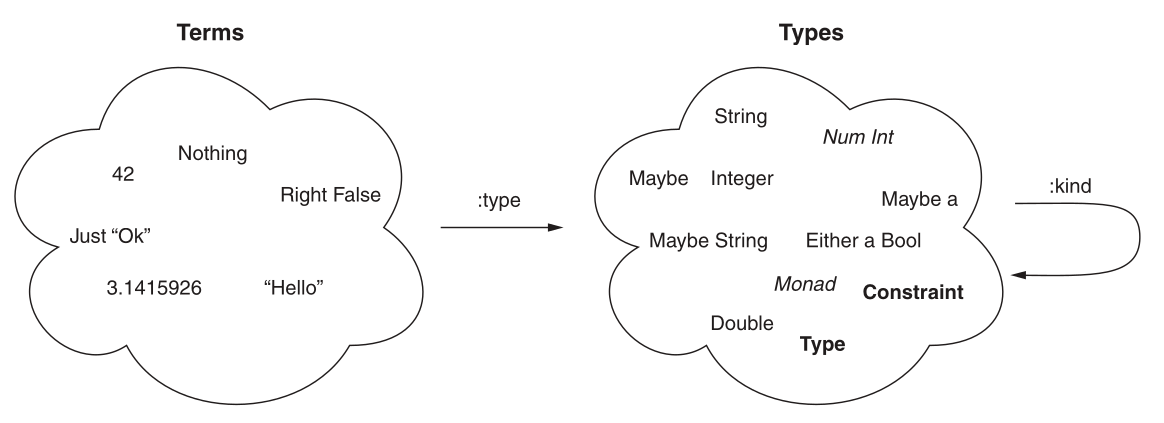
\includegraphics[width=0.99\textwidth]{figs/types-eq-kinds}
    \caption{Типы и канды --- одно~\cite{bragilevsky-haskell}.}
    \label{fig:types-eq-kinds}
\end{figure}

\subsection{Реализация параметрического полиморфизма}

\vocab{Конвенция вызова}\footnote{\url{https://en.wikipedia.org/wiki/Calling_convention}} представляет собой набор соглашений между тем как функция компилируется и как должна вызываться.
Например, функция принимает два аргумента, каждый размером в машинное слово, и возвращает один результат размером в машинное слово.
Тогда сгенерированный низкоуровневый код этой функции может, например, ожидать, что оба аргумента передаются через специальную пару регистров, а складывать результат он будет в третий.
В таком случае вызывающий код обязан предоставить аргументы в правильных регистрах и ожидать результата в некотором третьем, заранее оговоренном регистре.

В общем случае, конвенция вызова функции зависит от типов аргументов и результата.
Нужно знать как минимум их размер, чтобы понять, размещать их в регистрах или на стеке.
Нужно знать, это указатель (\vocab{reference type}) или значение само по себе (\vocab{value type}), чтобы понимать, как с ним работать.
В структурах данных нужно знать смещения полей.

Таким образом, реализация параметрического полиморфизма в языке --- это не тривиальная задача.
Разные языки используют различные подходы, все со своими достоинствами и недостатками.

\subsubsection{Mономорфизация} \label{subsubsec:monomorphization}

\vocab{Mономорфизация} --- самый прямолинейный подход, компилируем полиморфные функции и структуры для каждого набора типовых аргументов.
Так, если различных наборов типовых аргументов, с которыми эта функция вызывается, например, 100 (что запросто может быть), то её код будет компилироваться сто раз и занимать в бинарнике в сто раз больше места.
Так делают, например, C++ и Rust.

На самом деле всё ещё хуже.
Если проект многомодульный и состоит из множества единиц компиляции (кусков, которые компилируются отдельно), то одна и та же специализация функции на типовые аргументы будет компилироваться заново во всех единицах компиляции, где такая специализация нужна.
А затем, линкер будет заниматься удалением дубликатов, что тоже не самый быстрый и эффективный процесс.

\begin{itemize}
    \item[\positive] Порождаемый код максимально эффективен для каждого типа;
    \item[\positive] Легко на этапе компиляции отрабатывают \texttt{is}-проверки значений на принадлежность определённому типу (в остальных подходах с этим всё сложно);
    \item[\negative] Время компиляции крайне велико;
    \item[\negative] Существенно увеличивается размер результирующего бинарного файла, что может быть критично для некоторых приложений;
    \item[\negative] Может неэффективно работать из-за засорения кеша кода в процессоре;
    \item[\negative] В интерфейсах не может быть полиморфных методов, так как мы не знаем в месте вызова, к какому именно наследнику относится вызываемый метод, и какой код нужно специализировать (аналогично, не работает higher-rank полиморфзм);
    \item[\negative] К полиморфным функциям нельзя динамически линковаться (у них нет кода до специализации);
    \item[\negative] В общем случае нельзя поддержать variance, потому что код компилируется для конкретного типа и в общем случае не может работать для произвольного подтипа или супертипа (если reference и value типы могут находиться в одной иерархии подтипизации).
\end{itemize}

Некоторые языки не делают инстанциацию скрытой деталью реализации языка, а предоставляют её как инструмент пользователям.
Так делают, например, C++ и Zig.
А именно, это позволяет добиться следующего:
\begin{itemize}
    \item Если разрешить использовать значения в типах, инстанциация может использоваться как механизм вычислений на этапе компиляции.
    \item Если отложить проверку ошибок на стадию инстанциирования, то мы получим своего рода статическую утиную типизацию.
    Это позволит не описывать сложные сигнатуры полиморфных функций.
    Однако тогда функции для тестирования придётся вручную инстанциировать против всевозможных типов, иначе нельзя понять статически, компилируется она хотя бы против этих типов или нет.
\end{itemize}

% todo The Simple Essence of Monomorphization

\subsubsection{Стирание типа} \label{subsubsec:type-erasure}

Можно всё сделать наоборот, унифицировав значения, которые приходят на вход полиморфным функциям и хранятся в полиморфных структурах данных, вместо того, чтобы компилировать код под каждый тип.

Пусть каждое значение будет аллоцировано в куче и передаваться по указателю.
Тогда мы сможем переиспользовать один и тот же код для разных типовых аргументов --- он просто будет ожидать указатели.

\begin{itemize}
    \item[\positive] Каждая функция компилируется ровно один раз --- быстро;
    \item[\positive] Можно динамически загружать новые полиморфные функции и типы и использовать их друг с другом;
    \item[\positive] Гибкость --- вариантность, полиморфные методы в интерфейсах, higher-rank types и т.д. просто работают;
    \item[\negative] Аллокация в куче и разыменование указателя может очень сильно замедлить код;
    \item[\negative] Поскольку информация о типах стирается, нельзя ничего сделать с типовым аргументом, не имея его обитателей (например, запросить рефлексией информацию или сделать \texttt{is} проверку).
\end{itemize}

Такого подхода придерживаются JVM, Haskell и, как правило, другие функциональные языки ввиду его гибкости и скорости компиляции.

Особую проблему вызывает работа с примитивами и другими value-типами, потому что каждое значение приходится сначала боксить (переносить в кучу), а потом уже использовать в полиморфном контексте.
Поэтому языки борются с этим как могут.
Некоторые языки урезают диапазоны значений примитивов, чтобы зарезервировать бит, определяющий, это указатель или значение.
Код консультируется с этим битом для работы (похоже на~\ref{subsubsec:swift-generics}).
Так делают, например, OCaml и \href{https://koka-lang.github.io/koka/doc/book.html#sec-value-types}{Koka}.
Агрессивный инлайнинг тоже помогает.
Java пытается аккуратно двигаться в сторону возможности мономорфизации\footnote{\href{https://youtu.be/JI09cs2yUgY?si=MLkRs31mN1koXIu1}{Type Specialization of Java Generics - What If Casts Have Teeth ?}}\footnote{\url{https://cr.openjdk.org/~jrose/values/parametric-vm.html}}.

\subsubsection{Гибридный подход} \label{subsubsec:hybrid}

С\# реализует гибридный подход\footnote{\href{https://learn.microsoft.com/en-us/dotnet/csharp/programming-guide/generics/generics-in-the-run-time}{Generics in the runtime (C\# programming guide).}}.
Они различают значения, хранимые в куче --- reference types, и значения, хранимые на стеке --- value types.
Для первых они генерируют одну специализацию, работающую с указателями.
Для каждого набора value-типов они генерируют лениво в рантайме специализации.

То есть следы дженериков в таком подходе есть и промежуточном представлении CIL, и в рантайме.

\begin{itemize}
    \item[\positive] value-типы хранятся и передаются as-is без боксинга;
    \item[\positive] Доступна рефлексия по дженерикам;
    \item[\positive] Небольшое время компиляции;
    \item[\negative] Инстанциация в рантайме замедляет исполнение;
    \item[\negative] Variance работает только для reference types (что странно --- есть ``правильная'' подтипизация, а есть ``неправильная'').
\end{itemize}

\subsubsection{Использование виртуальной таблицы свойств типов} \label{subsubsec:swift-generics}

Swift\footnote{\href{https://youtu.be/ctS8FzqcRug?si=y_ZYnuUOulA33d_X}{(youtube) 2017 LLVM Developers’ Meeting: ``Implementing Swift Generics''}} вместе с каждым типовым параметром передаёт value witness table (рис.~\ref{fig:swift-witness-table}).
Это таблица со всей необходимой информацией, о типе: размер и выравнивание, что нужно сделать при копировании и перемещении объекта (например, инкрементировать счётчик ссылок).
Таким образом, скомпилированный код постоянно обращается к этой таблице и делает виртуальные вызовы функций из неё (рис.~\ref{fig:swift-generated-code}).
\begin{figure}
    \centering
    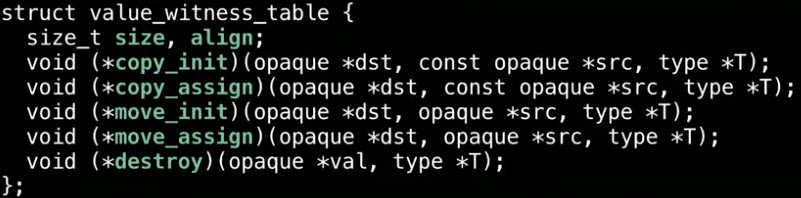
\includegraphics[width=0.7\textwidth]{figs/swift-witness-table}
    \caption{Swift value witness table.}
    \label{fig:swift-witness-table}
\end{figure}
\begin{figure}
    \centering
    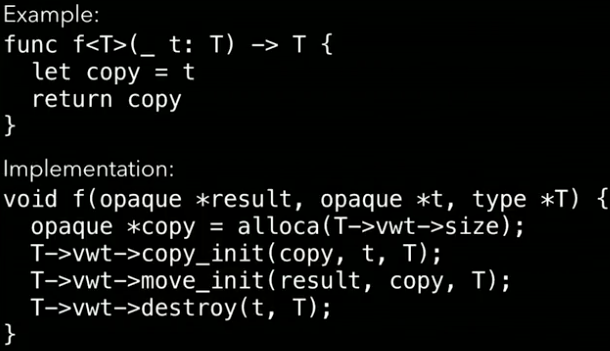
\includegraphics[width=0.5\textwidth]{figs/swift-generated-code}
    \caption{Код полиморфной функции, порождаемый компилятором Swift.}
    \label{fig:swift-generated-code}
\end{figure}

\begin{itemize}
    \item[\positive] Небольшое время компиляции;
    \item[\positive] Предсказуемая эффективность (не приводит к неожиданным паузам в рантайме);
    \item[\positive] Эффективная работа с value-значениями;
    \item[\positive] Высокая гибкость;
    \item[\positive] Информация о типах не стирается;
    \item[\negative] Серьёзный константный оверхед на динамические вызовы через таблицу, эффективность очень сильно зависит от компиляторных оптимизаций.
\end{itemize}

Своего рода реализация параметрического полиморфизма через специальный.

\subsection{Полиморфизм по конвенции вызова} \label{subsec:representation-polymorphism}

Как мы уже обсуждали выше~\ref{subsubsec:type-erasure}, параметрический полиморфизм в Haskell реализуется следующим образом: все значения хранятся в куче и передаются в полиморфные функции по указателю.
Однако, если для вычислительного кода важна производительность, такой подход не годится ввиду большой нагрузки на подсистему управления памятью и множества индирекций.
Поэтому Haskell позволяет также писать код с использованием unboxed значений.
А если конвенция вызова не принципиальна, можно по ней абстрагироваться и писать один код для boxed и unboxed значений~\cite{eisenberg2017levity}.

\subsubsection{Разновидности runtime представлений в Haskell}

\begin{figure}[h]
    \centering
    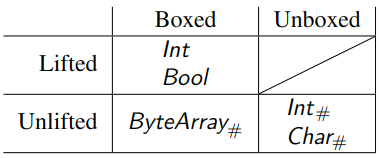
\includegraphics[width=0.5\textwidth]{figs/haskell-value-kinds}
    \caption{Виды значений в Haskell с примерами~\cite{eisenberg2017levity}.}
    \label{fig:haskell-value-kinds}
\end{figure}

На рисунке~\ref{fig:haskell-value-kinds} можно увидеть классификацию значений в Haskell с примерами типов.
\vocab{Unboxed типы} --- их значения удерживаются и передаются по значению.
\vocab{Boxed}, соответственно, наоборот, передаются по указателю и хранятся в куче.
Обычный \mintinline{haskell}|Int| является просто декларацией следующего вида, где \mintinline{haskell}|I#| --- это обычный конструктор с необычным именем, содержащий unboxed значение.
\begin{minted}{haskell}
    data Int = I# Int#
\end{minted}

\vocab{Lifted типы} --- содержат $\bot$ в качестве значения.
Иначе говоря, могут содержать отложенные вычисления (это для них специальным образом обеспечивают компилятор и рантайм).
\vocab{Unlifted типы} --- наоборот, не могут быть отложенными.
Операции, производящие значения unlifted типов всегда энергичные.
Свойство lifted/unlifted называют \vocab{levity}.
Чтобы распространить дальнейшее изложение на энергичные языки, можно levity заменить на boxity и всё останется справедливым.

\# в именах типов и функций --- это конвенция, показывающая, что где-то рядом происходит работа с unlifted значениями\footnote{Нужно подключить расширение \href{https://ghc.gitlab.haskell.org/ghc/doc/users_guide/exts/magic_hash.html}{MagicHash}, чтобы пользоваться \# в идентификаторах.}.

Также в Haskell есть unboxed кортежи, которых не существует на этапе исполнения.
Например, следующая функция как бы возвращает пару значений, но в действительности компилятор может их разместить, например, в паре регистров.
Соответственно, паттерн-матчинг по таким кортежам, просто позволяет сослаться на каждое из этих значений.
\begin{minted}{haskell}
    divMod# :: Int -> Int -> (# Int, Int #)
    case divMod# n k of (# quot, rem #) -> ...
\end{minted}
Соответственно, нет никакого различия между по-разному вложенными unboxed кортежами:
\begin{minted}{haskell}
    (# A, (# B, C #)) ?$\equiv$? (# #( A, B #), C #) ?$\equiv$? (# A, B, C #)
\end{minted}

\subsubsection{Классификация значений по runtime представлению}

Значения различных типов могут быть на этапе исполнения устроены по-разному.
То есть нам нужна некоторая система классификации типов.
Но такая система в Haskell уж есть --- кайнды.
Опишем в виде структур данных предметную область, а потом продвинем на нужный уровень с помощью DataKinds~\ref{subsubsec:promotion}.

Стандартная библиотека Haskell \href{https://downloads.haskell.org/ghc/latest/docs/users_guide/exts/representation_polymorphism.html}{предоставляет} следующие типы данных:
\begin{minted}{haskell}
    TYPE :: RuntimeRep -> Type

    data Levity = Lifted | Unlifted

    data RuntimeRep = BoxedRep Levity
                    | IntRep | DoubleRep
                    | TupleRep [RuntimeRep]
                    | SumRep [RuntimeRep]
                    | ...

    type LiftedRep = BoxedRep Lifted

    type Type = TYPE LiftedRep
\end{minted}

\mintinline{haskell}|TYPE| --- это магический тип, определённый в компиляторе.
Он параметризован runtime-представлением значений.
Теперь привычный \mintinline{haskell}|Type| --- это частный случай с boxed lifted значениями.

%! suppress = Quote
\begin{itemize}
    \item \mintinline{haskell}|Int :: TYPE (BoxedRep Lifted)| или \mintinline{haskell}|:: Type|
    \item \mintinline{haskell}|IntRep| и \mintinline{haskell}|DoubleRep| соответствуют представлению численных констант (в зависимости от архитектуры процессора, целые числа и числа с плавающей запятой может быть необходимо располагать в различных специальных регистрах)\\ \mintinline{haskell}|Int# :: TYPE IntRep|
    \item \mintinline{haskell}|Maybe Int :: Type|
    \item \mintinline{haskell}|Maybe :: Type -> Type|
    \item \mintinline{haskell}|TupleRep| и \mintinline{haskell}|SumRep| --- unboxed алгебраические типы, представления параметризованы представлениями хранимых значений\\
    \mintinline{haskell}|(# Int, Bool #) :: TYPE (TupleRep '[LiftedRep, LiftedRep])|
    \item Для простоты, типы вложенных кортежей не унифицируются
    \begin{minted}{haskell}
        (# Int#, (# Int, Double# #) #)
          :: TYPE (TupleRep '[IntRep, TupleRep '[LiftedRep, DoubleRep]])
    \end{minted}
\end{itemize}

\subsubsection{Representation polymorphism}

Выставив runtime-представление в структуре кайндов, мы теперь можем параметризоваться по ним.
Например, кайнд функциональной стрелки выглядит следующим образом\footnote{Выключить упрощения: \mintinline{haskell}|ghci> :set -fprint-explicit-foralls -fprint-explicit-runtime-reps|}:
\begin{minted}{haskell}
    ghci> :k (->)
    (->) :: forall {q :: RuntimeRep} {r :: RuntimeRep}. TYPE q -> TYPE r -> Type
\end{minted}

\begin{task}
    Подумайте, почему функция имеет boxed тип.
    Может ли быть иначе?
    Может ли это быть полезным?
\end{task}

К сожалению, Haskell выставляет довольно строгое ограничение: связыватели не могут иметь тип, полиморфный по runtime представлению.
Можно легко предположить, почему,~--- нельзя сгенерировать код функции для работы с параметром произвольного рантайм-представления.
Это можно решить только мономорфизацией~\ref{subsubsec:monomorphization}, но Haskell избегает этого подхода\footnote{\url{https://gitlab.haskell.org/ghc/ghc/-/issues/14917}}.
Сообщество также пытается найти другие решения\footnote{\url{https://mail.haskell.org/pipermail/haskell-cafe/2023-January/135770.html}} (что-то вроде~\ref{subsubsec:swift-generics}).

Например, изначально оператор аппликации был обобщён только по возвращаемому типу.
Это не порождает проблем, так как вызывающий код сможет вывести представление и сгенерировать подходящий код:
\begin{minted}{haskell}
    ($) :: forall r a (b :: TYPE r). (a -> b) -> a -> b
    f $ ?\framebox{x}? = f x
\end{minted}

Однако, было замечено, что для оператора аппликации можно получить другую реализацию, не использующую levity-полиморфное связывание\footnote{\url{https://gitlab.haskell.org/ghc/ghc/-/merge_requests/10131}}:
\begin{minted}{haskell}
    ($) :: forall ra rb (a :: TYPE ra) (b :: TYPE rb). (a -> b) -> a -> b
    ($) f = f
\end{minted}

Таким образом, в Haskell полиморфизм по представлениям несколько вырожден и помогает лишь в небольшом количестве случаев, однако немаловажных.
Если позволить мономорфизацию по \mintinline{haskell}{RuntimeRep} параметрам, получится система аналогичная гибридной реализации параметрического полиморфизма~\ref{subsubsec:hybrid}, только с большим контролем со стороны программиста над мономорфизацией.
